\chapter{\ifproject%
\ifenglish Project Structure and Methodology\else โครงสร้างและขั้นตอนการทำงาน\fi
\else%
\ifenglish Project Structure\else โครงสร้างของโครงงาน\fi
\fi
}

ในบทนี้จะกล่าวถึงหลักการ, การนำทฤษฎีที่เกี่ยวข้องมาประยุกต์ใช้ และการออกแบบของระบบ

\makeatletter

% \renewcommand\section{\@startsection {section}{1}{\z@}%
%                                    {13.5ex \@plus -1ex \@minus -.2ex}%
%                                    {2.3ex \@plus.2ex}%
%                                    {\normalfont\large\bfseries}}

\makeatother
%\vspace{2ex}
% \titleformat{\section}{\normalfont\bfseries}{\thesection}{1em}{}
% \titlespacing*{\section}{0pt}{10ex}{0pt}

\section{การจัดเก็บข้อมูล}
โดยข้อมูลราคาหุ้นทุกตัวจะมีแหล่งที่มาจาก 2 ที่ก็คือ AlphaVantage และ Finnhub โดย AlphaVantage จะให้ข้อมูลย้อนหลังไป 2 ปี ส่วน Finnhub จะเอาไว้ใช้อัพเดท
ข้อมูลแบบ real-time ทุกๆ 1 ชม. และในส่วนของราคา Crypto-Currency จะมีแหล่งที่มาจาก Binance ทั้งหมด
เราใช้ MongoDB เป็น Database สำหรับจัดเก็บข้อมูลตลาดหุ้น และตัวชี้วัดทางเทคนิคที่เราต้องการใช้ เช่น RSI, MA เป็นต้น

ในตอนเริ่มตันนั้นเราดึงข้อมูลที่ต้องการมาจาก AlphaVantage API ซึ่งได้มาเป็นข้อมูลตลาดหุ้นย้อนหลัง 2 ปีโดย
และเก็บข้อมูลลง MongoDB ด้วย Rust โดยมีการแปลงข้อมูลให้เป็นในรูปแบบข้อมูลตลาดของเราซึ่งก็จะประกอบด้วย
\begin{enumerate}
    \item ticker: ชื่อของหุ้นที่ทำการซื้อขาย เช่น AAPL/USD, TSLA/USD, ETH/USDT
    \item open: เป็นราคาซื้อขายแรกที่เกิดขึ้นใน ช่วงเวลานั้นๆ
    \item close: เป็นราคาสุดท้ายที่เกิดขึ้นจากการซื้อขายสิ้นสุด ของช่วงเวลานั้นๆ
    \item high: การเคลื่อนไหวของราคาหุ้น ณ ระดับราคาสูงสุดในช่วงเวลานั้นๆ
    \item low: การเคลื่อนไหวของราคาหุ้น ณ ระดับราคาต่ำสุดในช่วงเวลานั้นๆ
    \item volume: ปริมาณการซื้อขายในช่วงเวลานั้นๆ
\end{enumerate}
จากนั้นในการอัพเดตข้อมูลแบบ real-time เราจะใช้ MongoDB Scheduled Triggers ที่จะไปเรียกใช้ AWS Lambda ที่เราสร้างขึ้นมาโดยใน Lambda จะดึงข้อมูลจาก 
Finnhub มาอัพเดตที่จะมีการอัพเดตข้อมูลของตัวชี้วัดทางเทคนิคที่เราต้องการใช้ด้วย และอัพเดตตัวชี้วัดทางเทคนิคที่สร้างจาก fuzzy logic ของเราเองด้วย
ในส่วนของ Crypto-Currency ก็จะใช้ระบบแบบเดียวกันแต่จะใช้ Binance API ทั้งในการดึงข้อมูลครั้งแรกและการอัพเดตแบบ real-time

\begin{figure}[ht]
    \centering
    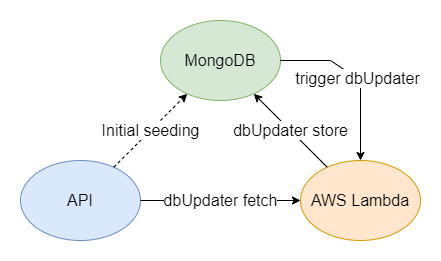
\includegraphics[scale=0.6]{images/db.png}
    \caption{โครงสร้างของการจัดเก็บข้อมูล โดนเส้นประคือทำครั้งเดียวในตอนแรกเริ่ม และเส้นทึบจะทำในทุกๆ ชม. โดยเป็นการเรียกใช้โปรแกรม dBUpdater ใน AWS Lambda}
    \label{fig:7}
\end{figure}
\FloatBarrier

\section{การสร้างตัวชี้วัดทางเทคนิคด้วย Fuzzy Logic}
เราจะใช้ Mamdani Fuzzy Inference System กับตัวแปรทางภาษาและ fuzzy rule ที่จะกล่าวด้านล่างนี้ในการคำนวณค่าสัญญาณของเรามา โดย defuzzification method จะใช้แบบ
centroid 

\subsection{ตัวแปรทางภาษา (Linguistic Variable)}
สำหรับตัวชี้วัดทางเทคนิคแต่ละตัวที่เรามีให้ได้แก่ Relative Index Strength (RSI), Bollinger Band, Moving Average Convergence/Divergence 
(MACD), Average Directional Index (ADX), Aroon oscillator, On-Balance Volume (OBV), Stochastic Oscillator, 
Accumulation/Distribution Indicator (A/D) เราจะมีตัวแปรทางภาษาสำหรับแต่ละตัวชี้วัดที่สอดคล้องกับการตีความทั่วๆไปของมัน
และเราก็จะมีตัวแปรทางภาษาที่ใช้ในการสร้างตัวชี้วัดทางเทคนิคใหม่ โดยเราจะทำป็นสัญญาณ long (ควรเข้า position long) และสัญญาณ short (ควรเข้า position short) โดยทั้ง long และ short
จะคิดมาจากตัวชี้วัดทางเทคนิคที่กล่าวถึงด้านบน ยกตัวอย่างตัวแปรทางภาษาที่เราอาจจะใช้บนรูปที่ \ref{fig:8} โดนในระบบผู้ใช้ก็จะสามารถปรับแต่งตัวแปรทางภาษาเหล่านี้ได้ตามต้องการของตัวเองผ่าน website 
และ mobile application

\begin{figure}[ht]
    \centering
    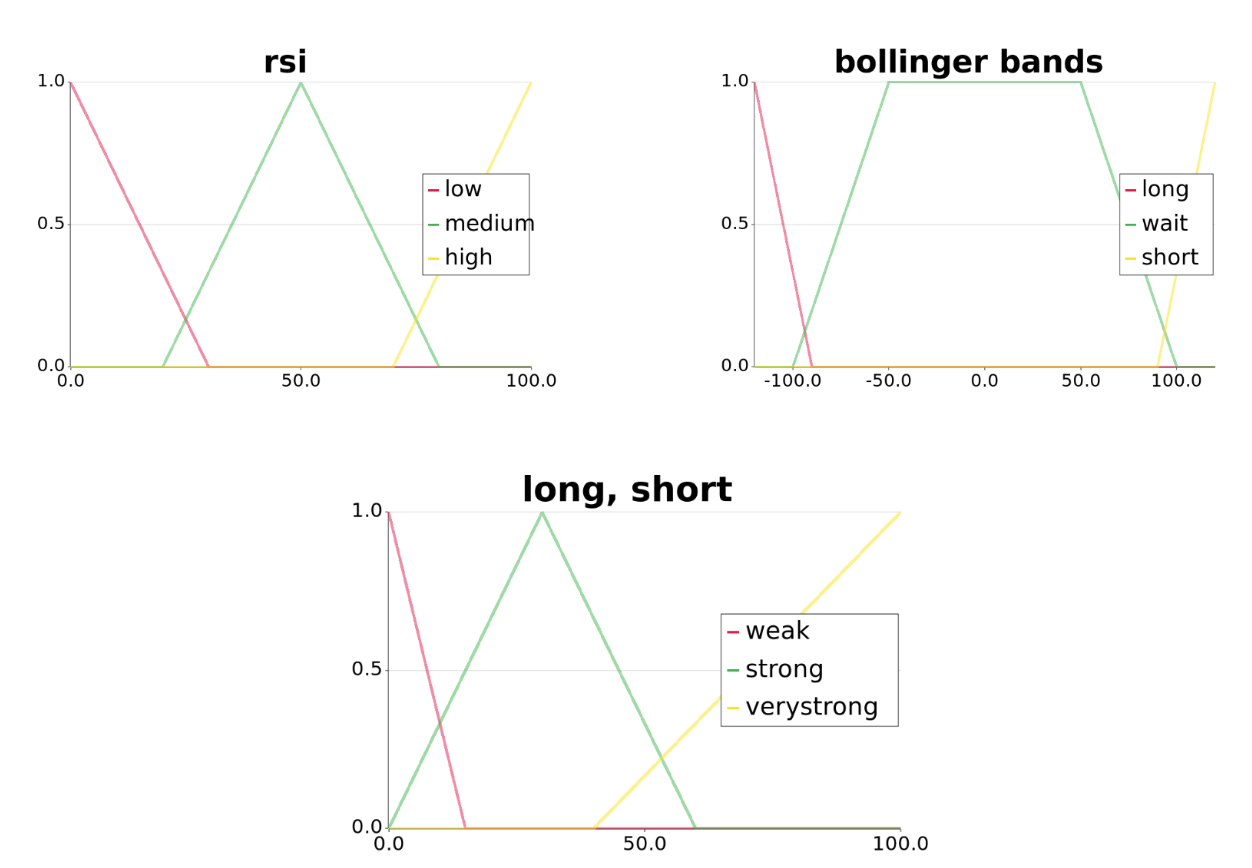
\includegraphics[width=\textwidth]{images/linguistic.png}
    \caption{ตัวแปรทางภาษาสำหรับ RSI, Bollinger Band, long, short}
    \label{fig:8}
\end{figure}

\subsection{Fuzzy Rules}
เราจะใช้การตีความทั่วๆไปของแต่ละตัวชี้วัดมาสร้าง Fuzzy Rule เริ่มต้น ยกตัวอย่างเช่นถ้าเราใช้แค่ RSI และ Bollinger Band ในการสร้าง long และ short เราจะมี fuzzy rule 
เหมื่อนในตารางที่ \ref{table:1} โดยในระบบของเราจริงๆ เราจะใช้ตัวแปรทางภาษาที่เรากล่าวในหัวข้อก่อนหน้ามาทั้งหมดสร้าง Fuzzy Rule ในการสร้างสัญญาณ long และ short และเรา
จะออกแบบระบบให้ผู้ใช้สามารถปรับแต่งกฏตรงนี้ได้ในทั้ง website และ mobile application

\begin{table}[htp]
	\centering
	\begin{tabular}{c c c c}
		\toprule
        {RSI} & {Bollinger Bands} & {LONG} & {SHORT} \\ 
        \midrule
        HIGH & LONG & WEAK & WEAK \\
        HIGH & WAIT & WEAK & STRONG \\
        HIGH & SHORT & WEAK & VERYSTRONG \\
        MEDIUM & LONG & WEAK & STRONG \\
        MEDIUM & WAIT & WEAK & WEAK \\
        MEDIUM & SHORT & STRONG & WEAK \\
        LOW & LONG & VERYSTRONG & WEAK \\
        LOW & WAIT & STRONG & WEAK \\
        LOW & SHORT & WEAK & WEAK \\
        \bottomrule
    \end{tabular} 
    \caption{ตัวอย่างของ Fuzzy Rules ที่ใช้แค่ RSI และ Bollinger Band เพื่อสร้าง long และ short.}
	\label{table:1}
\end{table}
\FloatBarrier

\section{การปรับแต่ง Fuzzy Logic ด้วย PSO}
เป้าหมายของเราในการปรับแต่ง Fuzzy Logic ที่ใช้สำหรับการสร้างตัวชี้วัดทางเทคนิคใหม่ของเรานั้น ก็คือการปรับแต่งตัวแปรทางภาษาต่างๆ ที่มีอยู่ fuzzy rules เพื่อให้
ตัวชี้วัดทางเทคนิคของเรานั้นสามารถสร้างกำไรได้มากที่สุดใน\emph{วิธีการเทรดที่เราใช้ปรับแต่ง} โดยเราจะใช้ PSO (Particle Swarm Optimization) ในการปรับพารามิเตอร์ที่ใช้
สร้าง linguistic variable แต่ละอัน โดยพารามิเตอร์ในการสร้าง fuzzy set นั้นจะแตกต่างกันไปตามรูปแบบของ fuzzy set 
เช่นถ้าเป็นแบบสามเหลี่ยมก็จะมีพารามิเตอร์ดังที่เห็นในรูปที่ \ref{fig:9} โดยเราจะทำการปรับแต่งนี้และบันทึก fuzzy rules ใหม่ในฐานข้อมูลของเราทุกๆ เดือน

\begin{figure}[ht]
    \centering
    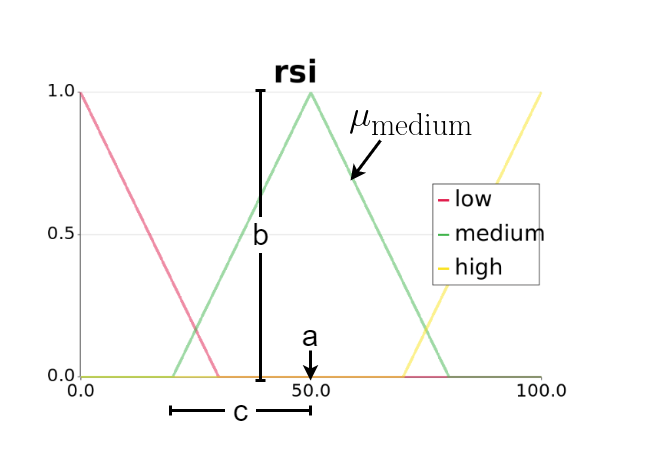
\includegraphics[width=0.8\textwidth]{images/linguisticv.png}
    \caption{ตัวแปรทางภาษาและตัวแปรที่เราต้องการจะปรับแต่ง $\mu_{\text{medium}} = b (1 - \frac{ |x-a| }{s})$ (ในที่นี้คือเราจะปรับแต่งค่าของ $a, b, s$)}
    \label{fig:9}
\end{figure}

\subsection{กลยุทธ์ที่เราใช้ปรับแต่ง}
โดยในการปรับแต่ง Fuzzy Logic ของเรานั้นอันดับแรกเลยเราต้องเลือกกลยุทธ์การเทรดที่เราต้องการปรับแต่ง ให้มีผลต่อตัวชี้วัดทางเทคนิค ยกตัวอย่างกลยุทธ์การเทรด
เช่น มีเงินต้น 2000 บาท ถ้า buySignal มากกว่า 50 ให้เข้าซื้อด้วย 100 บาท ด้วย stop-loss ที่ 10\% และ take profit ที่ 20\% 
\subsection{Backtesting}
Backtesting คือการนำกลยุทธ์การเทรดที่เราเลือก ไปใช้กับข้อมูลในอดีตในกรอบเวลาที่ผ่านๆ มาเพื่อทดสอบว่ากลยุทธ์นั้นไปใช้ในตลาดจริงๆ ในอดีตแล้วได้ผลดีแค่ไหน
โดยเราสามารถเลือกกรอบเวลาที่ตลาดมีลักษณะคล้ายๆ กับในปัจจุบัน แล้วลองปรับเปลี่ยนและทดสอบกลยุธ์การเทรดนั้นๆ ได้เพื่อให้ได้ผลลัพธ์ที่เราต้องการ

โดยเราจะทำการ backtest ด้วยกลยุทธ์การเทรดที่เราเลือกมา แล้วเก็บข้อมูลการเทรดที่เกิดขึ้นทั้งหมดโดยแต่ละการเทรดจะมีข้อมูลดังนี้ 
\begin{itemize}
    \item เวลาที่เข้า position
    \item เวลาที่ออก position
    \item ราคาที่เข้าซื้อ
    \item ราคาที่ขาย
    \item จำนวนเงินที่จ่ายไป
    \item กำไรขาดทุนที่ได้ ($\text{realizedPnl}$)
\end{itemize}

\subsection{Objective Function}
เราจะใช้ Objective Function ที่คำนวณมาดังนี้ $f = \text{NP} - \text{MDD}$ โดย
\begin{itemize}
    \item {$\text{NP} = \frac{\sum_{i=0}^{n} p_i(\text{realizedPnl})}{\text{startMoney}}$ 
        คือ Net Profit ที่มีค่าอยู่ในช่วง $[0, \infty)$ ซึ่งได้จากการเทรดทั้งหมดโดยคำนวนจากข้อมูลการเทรดที่เราได้จากการทำ backtest โดย $n$ คือจำนวนข้อมูลทั้งหมด
        และ $p_i(\text{realizedPnl})$ คือข้อมูลตัวที่ $i$ โดยเอาค่า $\text{realizedPnl}$ มา 
    }
    \item {$\text{MDD}$ (Maximum Drawdown ตัวอย่างในรูปที่ \ref{fig:10}) มีค่าอยู่ในช่วง $[0, 1]$ โดยเราสามารถคิดค่านี้โดยให้ 
    $$
        g(x) = \sum_{i = 0}^{x}p_i(\text{realizedPnl})
    $$
    \begin{equation}
        \text{MDD}' = \max_{r \in (0, n)} \left[ \max_{t \in (0, r)} g(t) - g(r) \right]
    \end{equation}
    แล้วให้เราจำค่า $y = g(t)$ ที่ทำให้ได้ 
    $\text{MDD}'$ เยอะที่สุดไว้ แล้วจะได้ว่า $\text{MDD} = \frac{\text{MDD}'}{y}$
    }
\end{itemize}
ในส่วนของ hyper parameters ต่างๆ ที่เราต้องตั้งให้ PSO algorithm เช่น จำนวน particles, การคำนวณ velocity เป็นต้น จะเปลี่ยนไปตามแต่ละครั้งของการปรับแต่ง 
โดยเราจะทดลองหลายๆ แบบเพื่อให้ได้ตัวชี้วัดที่มีประสิทธิภาพดีที่สุด

\begin{figure}[ht]
    \centering
    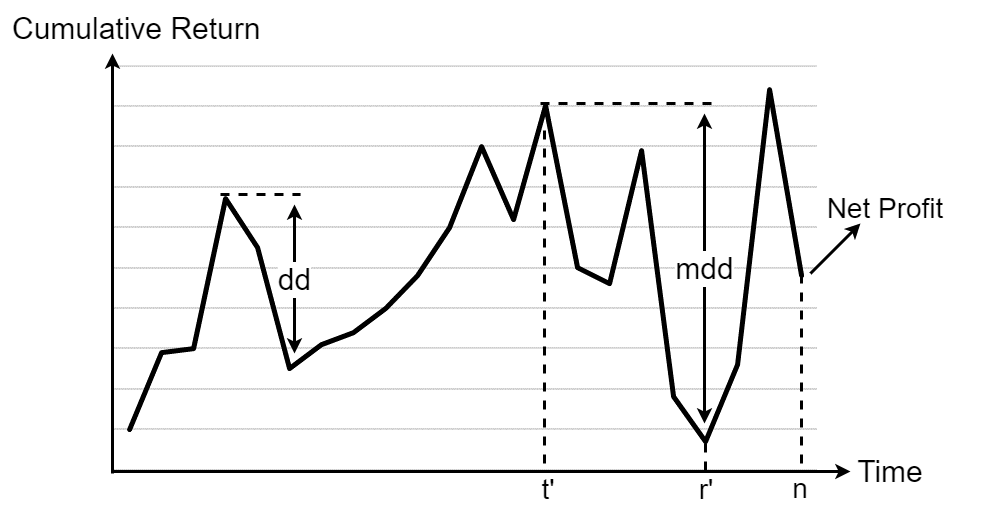
\includegraphics[width=0.8\textwidth]{images/mdd.png}
    \caption{ตัวอย่างของ Net Profit และ Maximum Drawdown}
    \label{fig:10}
\end{figure}

\section{การจัดการเงินทุน}
เราจะใช้ optimal-f (\cite{Vince}) ที่ถูกดัดแปลงตามที่ \cite{Rodrigo} ได้ทำไว้ในส่วนของการจัดการเงินทุน ซึ่งจะบอกเราว่าควรลงทุุนโดยใช้เงินเท่าไหร่ เพื่อให้เงินกำไรเติบโตแบบ
geometric โดยจะคิดมาจากผลลัพธ์ของการเทรดก่อนหน้า ถ้าเราเทรดสำเร็จเยอะก็จะเพิ่มเงินที่จะลงทุน ถ้าเทรดพลาดเยอะก็จะลดเงินที่จะลงทุน 

อันดับแรกให้เราหาค่า $f$ ที่ทำให้ terminal wealth relative ($\text{TWR}$) ในสมการ \ref{eq:twr} มีค่ามากที่สุด
\begin{equation}
    \text{TWR}(f) = \Pi_{i=1}^{n} \text{HPR}_i(f)
\label{eq:twr}
\end{equation}
\begin{equation}
    \text{HPR}_i(f) = 1 + \frac{f \cdot p_i(\text{realizedPnl})}{\text{riskFactor}}
\end{equation}
โดยที่ $\text{HPR}$ คือ holding perioid return หรือก็คืออัตราส้วนกำไรขาดทุนของแต่ละ position 
,$n$ คือจำนวน position ทั้งหมด, $p_i(\text{realizedPnl})$ คือกำไรขาดทุนของ position ที่ $i$, 
และ $\text{riskFactor}$ คือค่าสัมบูรณ์ของ $p_i(\text{realizedPnl})$ ที่แย่ที่สุด

แต่ในปรกติแล้วค่า $f$ ที่เราได้มานั้นจะมีความเสี่ยงมากเกินไปเราก็จะใช้เป็น liquid-F ที่เป็น 10\% ของ $f$ เป็น $\text{liquid}_f = 0.1f$ 
\begin{equation}
\text{size} = \text{liquid}_f + \frac{(\text{output} - \text{threshold}) \cdot (f - \text{liquid}_f)}{\text{output}_{\text{max}} - \text{threshold}}
\end{equation}
โดย $\text{output}$ คือค่าจากสัญญาน long หรือ short ของเรา, $\text{threshold}$ คือค่าที่ $\text{output}$ ที่ต่ำที่สุดที่เราจะเข้า position, และ 
$\text{output}_{\text{max}}$ คือค่าที่มากที่สุดที่เป็นไปได้ของ $\text{output}$ จากนั้นเราก็นำ $\text{size}$ ไปคำนวณจำนวนที่จะลงทุนด้วยสมการ \ref{eq:shares}
\begin{equation}
\text{amount} = \frac{C \cdot \text{size}}{\text{price}}
\label{eq:shares}
\end{equation}
โดย $C$ คือจำนวนเงินที่เราทำไปลงทุนได้ และ $\text{price}$ คือราคาของสินทรัพย์ที่เราจะลงทุน แล้วถ้าเรามี $C$ ไม่พอให้เราลงทุนมากที่สุดเท่าที่จะทำได้

\section{เว็บเซิร์ฟเวอร์}
ก่อนจะเรียกใช้ APIs ต่างๆของเรานั้นผู้ใช้ต้องทำการสร้างบัญชีเอาไว้ก่อนเพื่อให้สามารถเก็บค่าการปรับแต่ง fuzzy logic ที่ผู้ใช้แต่ละคนทำไว้ได้ แล้ว endpoints แต่ละอันนั้นก็ต้องส่ง token ยืนยันตัวผู้ใช้
มาด้วย โดยเราจะมี endpoints ดังต่อไปนี้
\begin{enumerate}
    \item \texttt{GET /api/ohlc?symbol=xxx} จะให้ข้อมูล OHLC ของสินทรัพย์ที่เราต้องการ
    \item \texttt{GET /api/indicator?symbol=xxx\&type=xxx} จะให้ข้อมูลของตัวชี้วัดทางเทคนิคที่เราต้องการเช่น RSI, MACD, และอื่นๆที่กล่าวไป
    \item \texttt{GET /api/tunedfuzzy?symbol=xxx} จะให้ข้อมูลของตัวชี้วัดที่สร้างขึ้นมาด้วย fuzzy logic และถูกปรับแต่งด้วย PSO แล้ว
    \item \texttt{GET /api/fuzzy?symbol=xxx} จะให้ข้อมูลของตัวชี้วัดที่สร้างขึ้นด้วย fuzzy logic ที่ใช้กฏต่างๆ ที่ผู้ใช้ปรับแต่งไว้
    \item \texttt{GET /api/size} จะให้ค่า $\text{size}$ ในหัวข้อการจัดการเงินทุนมา เพื่อเอาไว้แนะนำขนาดของ position
    \item \texttt{POST /api/fuzzy} ใช้ปรับกฏและตัวแปรทางภาษาของ fuzzy logic
\end{enumerate}

\section{การพัฒนาเว็บไซต์และแอปพลิเคชันโทรศัพท์}
จุดประสงค์ของเว็บไซต์และแอปโทรศัพท์คือเป็นส่วนติดต่อให้กับผู้ใช้งานที่ต้องการเข้ามาใช้ระบบของเราโดยมีส่วนที่ต้องรองรับหลักดังนี้
\begin{itemize}
    \item ผู้ใช้งานสามารถดูกราฟ OHLC ของสินทรัพย์
    \item ผู้ใช้งานสามารถเพิ่มเครื่องมือตัวชี้วัดเบื้องต้นที่ต้องการอย่างเช่น RSI, MACD, และตัวอื่นๆที่ระบบของเรามีให้
    \item ผู้ใช้งานสามารถปรับแต่งระบบ Fuzzy logic (ปรับกฏ และตัวแปรทางภาษา)
    \item ผู้ใช้งานสามารถดูผลลัพธ์ที่ได้จากระบบ Fuzzy logic
\end{itemize}
ทำการออกแบบ UI/UX ของเว็บไซต์และแอปพลิเคชันโทรศัพท์ด้วย Figma
โดยในการพัฒนาเว็บไซต์ส่วนหลักใช้ UI Framework อย่าง SvelteKit และภาษา TypeScript ส่วนของที่เป็นแอปพลิเคชันโทรศัพท์จะใช้งาน Flutter และภาษา Dart

\section{แผนภาพกระแสข้อมูลโดยรวมของระบบ (Data Flow Diagram)}
แผนภาพแสดงกระแสข้อมูลโดยเริ่มตั้งแต่การดึงข้อมูลตลาดจาก API มาเก็บที่ Database ซึ่งข้อมูลในนั้นจะถูกนำมาใช้งานคำนวณตัวชี้วัดทางเทคนิค, ประมวลผลและปรับตั้งระบบฟัซซี จนกระทั่งได้สัญญาณจากระบบฟัซซีไปแสดงบนเว็บไซต์และแอปพลิเคชันบนมือถือให้กับผู้ใช้งาน
\begin{figure}[ht]
    \centering
    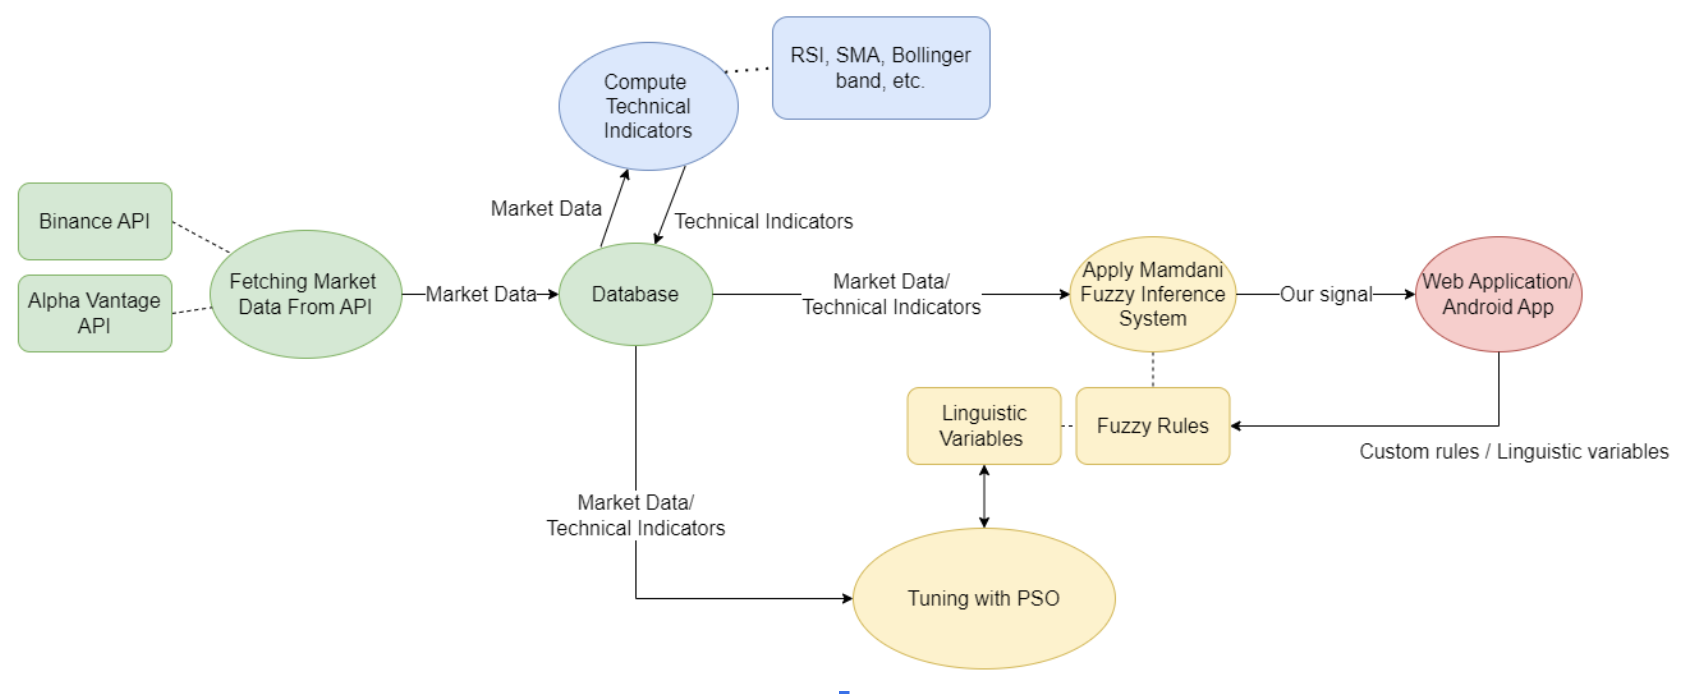
\includegraphics[scale=0.3]{images/overview.png}
    \caption{แผนภาพกระแสข้อมูล}
    \label{fig:11}
\end{figure}